\mychapter{Fundamentação Teórica}{cap:fundamentacao}

Para que se obtenha uma melhor compreensão acerca do tema proposto, neste  capítulo  será  apresentada  a  fundamentação teórica, a qual foi obtida por meio da revisão bibliográfica dos conceitos e técnicas presentes no estado da arte.

\section{Introdução às imagens SAR}

Como brevemente discutido no capítulo~\ref{cap:fundamentacao}, um RADAR consiste de um dispositivo capaz de detectar um objeto (alvo), indicando a sua distância e sua posição. Nesse contexto, segundo \citet{dissert_torres}, a maioria dos radares imageadores aerotransportados utilizados em sensoriamento remoto são os de visão lateral (\textit{Side-Looking Airborne Radar}). Nesse contexto, existem dois tipos de radar imageador: (i) o de abertura real (\textit{Real Aperture Radar} - RAR) e (ii) o de abertura sintética (SAR). Este último foi utilizado neste trabalho. Ademais, o tipo de detecção do sinal de retorno em um sistema SAR convencional pode ser linear ou quadrático. Deste modo, a imagem do terreno pode ser formada tanto em amplitude (detecção linear) quanto em intensidade (detecção quadrática) \citep{dissert_lucca}. 

Nesse cenário, o imageamento por RADAR consiste na emissão de pulsos de microondas a intervalos regulares sobre a região alvo e da recuperação dos sinais de retorno (\textit{backscatter}) provenientes da interação entre os pulsos eletromagnéticos e a região alvo à medida que o sensor se desloca.  

Estudos feitos por \citet{Clutter1997} e \citet{Gao2010StatisticalMO} caracterizam as regiões de imagens SAR quanto ao grau de homogeneidade apresentado e são elencadas nos seguintes tipos:
\begin{itemize}
    \item \textbf{Homogênea:} Caracterizada por um sinal de retorno sem alta variabilidade. Áreas de campos e pastagens, lagos e oceanos, representam, no geral, regiões homogêneas.
    \item \textbf{Heterogêneas:} Caracterizada por um sinal de retorno com significativa variabilidade. Regiões de florestas podem ser exemplos de regiões heterogêneas.
    \item \textbf{Extremamente Heterogêneas:} Caracterizada pela alta variabilidade do sinal de retorno. Esse tipo de homogeneidade é utilizada para modelar áreas urbanas, onde o espalhamento do terreno é bastante complexo.
\end{itemize}

Todos os processos para formação de imagens com iluminação coerente, como aqueles empregados por laser, ultrassom-B, sonar e radar de abertura sintética, sofrem uma espécie de degradação granular, chamada de \textit{speckle}. Este fenômeno, caracterizado como ruído, no contexto das imagens SAR ocorre devido à interferência construtiva e destrutiva das ondas coerentes refletidas pelos dispersores. Na seção seguinte serão discutidos tópicos referentes à modelagem estatística considerados clássicos de imagens SAR.


\section{Modelagem estatística e análise de dados SAR}

A estatística, de um modo geral, visa prover modelos e métodos que descrevam um determinado conjunto de dados \citep{dissert_torres}. O artigo de pesquisa de \citet{Gao2010StatisticalMO} discute em detalhes vários modelos estatísticos para esse tipo de dado e o autor ressalta que a modelagem estatística dos dados é essencial para interpretar imagens SAR, com o objetivo de descrevê-las e representar as características intrínsecas a estes dados.

Segundo \citet{Mejail2002}, dentre os modelos estatísticos disponíveis para modelagem e análise de imagens SAR, o modelo multiplicativo é muito preciso e bem-sucedido, baseando-se no pressuposto de que o campo aleatório observado (retorno) $Z$ é o resultado do produto de dois campos aleatórios independentes e não observados: $X$ e $Y$. O campo aleatório $X$ modela o retroespalhamento (\textit{backscatter}) do terreno e, portanto, depende apenas do tipo de área a que cada pixel pertence. O campo aleatório $Y$ leva em consideração que as imagens SAR são o resultado de um sistema de geração de imagens coerente que produz o conhecido fenômeno ruído \textit{speckle}, e que elas são geradas pela média de $n$ imagens (teoricamente independentes) - \textit{looks} - para reduzir o efeito do \textit{speckle}.

Então, nesse contexto, o Modelo Multiplicativo se mostra adequado para modelagem de dados SAR, já que o modelo empregado  deve ser capaz de separar tal ruído do que seria efetivamente a resposta do alvo na direção do sensor (\textit{backscatter}) e o presente modelo atende à essa restrição, sendo o modelo mais utilizado para modelar dados SAR. 

Conforme proposto e avaliado por \citet{Clutter1997}, a família de distribuições $G$ pode ser utilizada com sucesso para descrever os dados contaminados pelo ruído (\textit{speckle}) e, assim, a apresenta como "Modelo Universal" já que, através dela, é possível realizar a modelagem de dados SAR para o caso geral (regiões com diferentes graus de homogeneidade). Dessa forma, os dados ruidosos foram descritos no modelo multiplicativo usando a família $G$ de distribuições que é capaz de descrever áreas extremamente  melhor que a distribuição $K$. Nesse contexto, existem os casos especiais mais simples que têm se mostrado úteis na modelagem de áreas com diferentes graus de homogeneidade, como é o caso da distribuição $G_I^0$, e possuem a vantagem de tornar menos complicada a estimação dos parâmetros das distribuições. 


\subsection{Introdução à distribuição $G_I^0$}

Segundo \citet{FreryStochasticDistances2015}, o modelo $G_I^0$ é indexado por três parâmetros: o número de \textit{Looks} ($L$) que pode ser estimado em toda a imagem, um parâmetro de escala denotado por $\gamma$ e o parâmetro de rugosidade ou textura ($\alpha$). Este último está intimamente relacionado ao número de \textit{backscatters} elementares em cada pixel, uma das razões para receber atenção na literatura. Embora haja esforços em fornecer estimativas aprimoradas e robustas para tal quantidade, sua estimativa confiável ainda apresenta problemas numéricos na prática.

Vale ressaltar ainda que o número de \textit{Looks} consiste em um parâmetro que pode ser controlado no processo de geração de imagens e, portanto, será considerado conhecido. Este parâmetro está relacionado à relação sinal-ruído e à precisão espacial da imagem. Nesse contexto, conforme explica \citet{dissert_torres}, a principal finalidade do processamento \textit{Multilook} na geração de imagens consiste de reduzir o nível de ruído \textit{speckle} no momento da formação de imagens SAR. 

\subsection{Geração e caracterização de variáveis aleatórias $G_I^0$}

Como discutido anteriormente, no Modelo Multiplicativo há a suposição de que o valor observado em cada pixel é a ocorrência de uma variável aleatória $Z$, formada pelo produto de duas variáveis aleatórias independentes, a primeira delas é dada por $X$ que consiste na variável aleatória que modela o \textit{backscatter} e a segunda é dada por $Y$ que consiste na variável aleatória que modela o \textit{speckle}.

Conforme \citet{FreryStochasticDistances2015}, para dados SAR monopolarizados e no caso da distribuição $G_I^0$, o \textit{speckle} é modelado como uma variável aleatória \textit{Gama} ($\Gamma$), com parâmetro de forma $L \geq 1$, que corresponde ao número de \textit{Looks}, e média unitária, ou seja, o \textit{speckle} (Y) é modelado seguindo a distribuição dada por $\Gamma(L,1)$. O \textit{backscatter} (X), por sua vez, é modelado obedecendo a uma recíproca da lei \textit{Gama}, isto é, $\Gamma^{-1}(\alpha,\gamma)$. Com base nessas diretrizes provenientes do Modelo Multiplicativo, foi possível construir um método de geração variáveis aleatórias $G_I^0$, representadas pelo retorno $Z$, bastante útil nas simulações que foram realizadas ao longo deste trabalho, haja vista que a geração de variáveis aleatórias é imprescindível em qualquer programa de simulação.

Desse modo, temos que, se $Z \sim G_I^0(\alpha, \gamma, L)$, então sua função de densidade de probabilidade é dada por
\begin{equation}
    f_Z(z; \alpha, \gamma, \textit{L})= \frac{L^L\Gamma(L-\alpha)z^{L-1}}{\gamma^\alpha\Gamma(-\alpha)\Gamma(L)(\gamma + zL)^{L-\alpha}} \label{eq:fdpGI0}
\end{equation}
onde $-\alpha$, $\gamma$, $z$ > $0$ e $L \geq 1$. $\Gamma$, neste caso, representa a função \textit{gama}. Os parâmetros $\alpha$ e $\gamma$ nesta função de densidade são os parâmetros desconhecidos.

Por sua vez, os momentos de ordem $r$ ($r$-order moments) são dados por
\begin{equation}
    E(Z^r) = \left (\frac{\gamma}{L}\right )^{r}\frac{\Gamma(-\alpha-r)\Gamma(L+r)}{\Gamma(-\alpha)\Gamma(L)} \label{eq:moments}
\end{equation}
fornecidos dessa forma se $\alpha$ < $-r$, e são infinitos, caso contrário.

No processo de estimação, podemos fazer simplificações para reduzir a complexidade dos cálculos e tornar os resultados comparáveis, como assim foi feito no trabalho de \citet{FreryStochasticDistances2015}. Para isso, por exemplo, podemos escolher o parâmetro de escala ($\gamma$) de modo que se tenha $E(Z) = 1$, que é dado por $\gamma^{*} = -\alpha - 1$. Dessa forma, mantém-se o foco apenas no parâmetro $\alpha$ que é o que interessa neste trabalho.

Uma característica crucial da distribuição caracterizada por \eqref{eq:fdpGI0} é que seus parâmetros são interpretáveis: $\gamma$ é um parâmetro de escala e o número de \textit{Looks} é conhecido antecipadamente ou é estimado para a imagem inteira usando alvos estendidos (amostras muito grandes). Uma das características mais importantes da distribuição $G_I^0$ é a interpretação de seu parâmetro $\alpha$ que está relacionado com a rugosidade ou homogeneidade do alvo. Valores próximos de $0$, tipicamente maiores que $-3$, sugerem alvos extremamente texturizados ou heterogêneos, como zonas urbanas. Em situações intermediárias, à medida que o valor diminui, há o indicativo de regiões com textura moderada ou heterogêneas e produzem geralmente $\alpha$ $\in$ [$-6$,$-3$]. Exemplos de regiões desse tipo são as áreas irregulares, como zonas florestais. Alvos sem textura ou homogêneos geralmente produzem $\alpha \in (-\infty, -6)$ como é o caso de regiões lisas, por exemplo, pastagem, culturas e campos queimados. Esta é a razão pela qual a precisão na estimativa do parâmetro $\alpha$ é tão importante.

A figura a seguir apresenta as curvas de densidade da distribuição $G_I^0$ para determinados parâmetros.
% GI0 Densities
\begin{figure}[H]
     \centering
     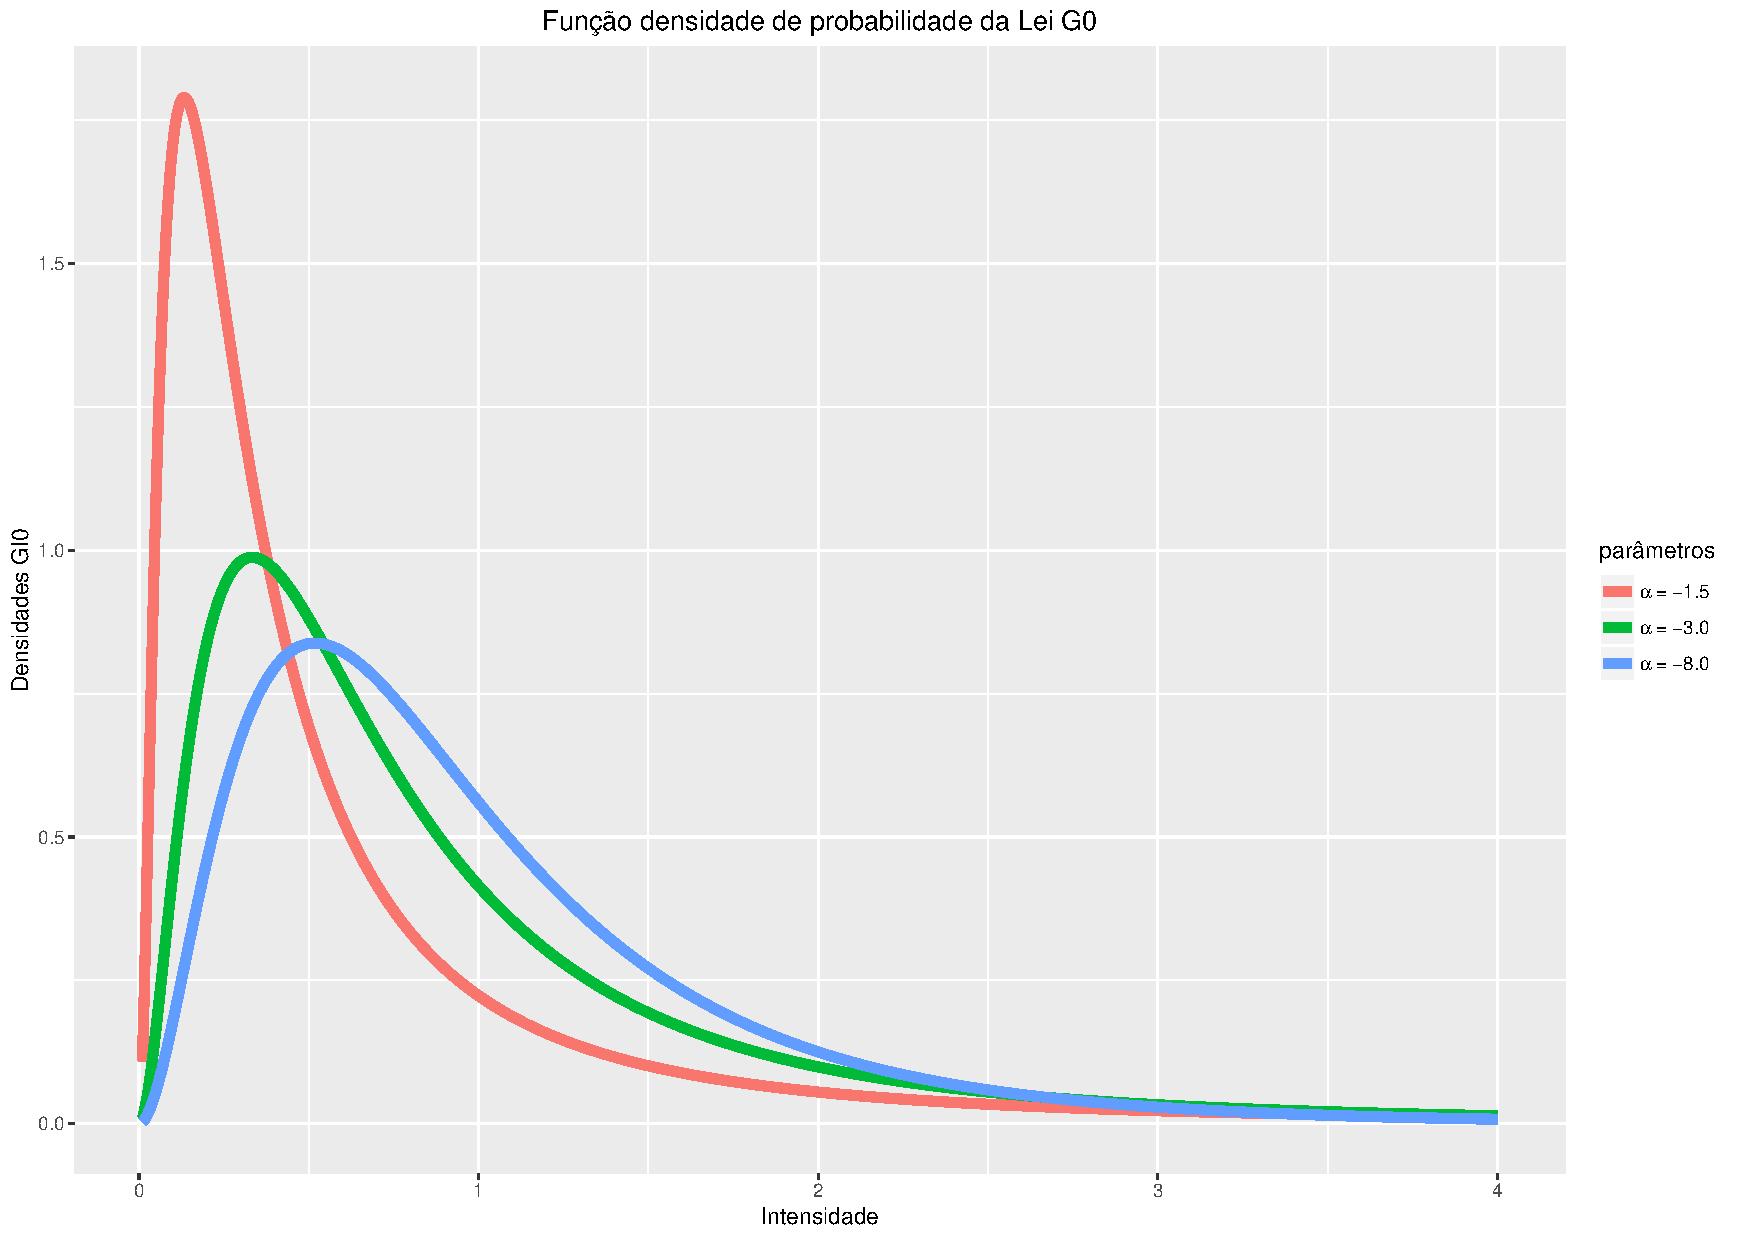
\includegraphics[scale=0.5]{plots/GI0Densities.pdf}
     \caption{Densidades da distribuição $G_I^0(\alpha, -\alpha - 1, 3)$, com $\alpha \in \left \{  -8.0, -3.0, -1.5 \right \}$}
     \label{graf_1}
\end{figure}

Já na figura abaixo temos o resultado do histograma feito a partir de um conjunto de $10.000$ variáveis aleatórias $G_I^0$ geradas a partir da função que segue o Modelo Multiplicativo, conforme explicado anteriormente. Juntamente a esse histograma, temos o traçado da curva de densidade de probabilidade e, com isso, é possível perceber um determinado ajuste entre ambos.
% GI0 Generation
\begin{figure}[H]
     \centering
     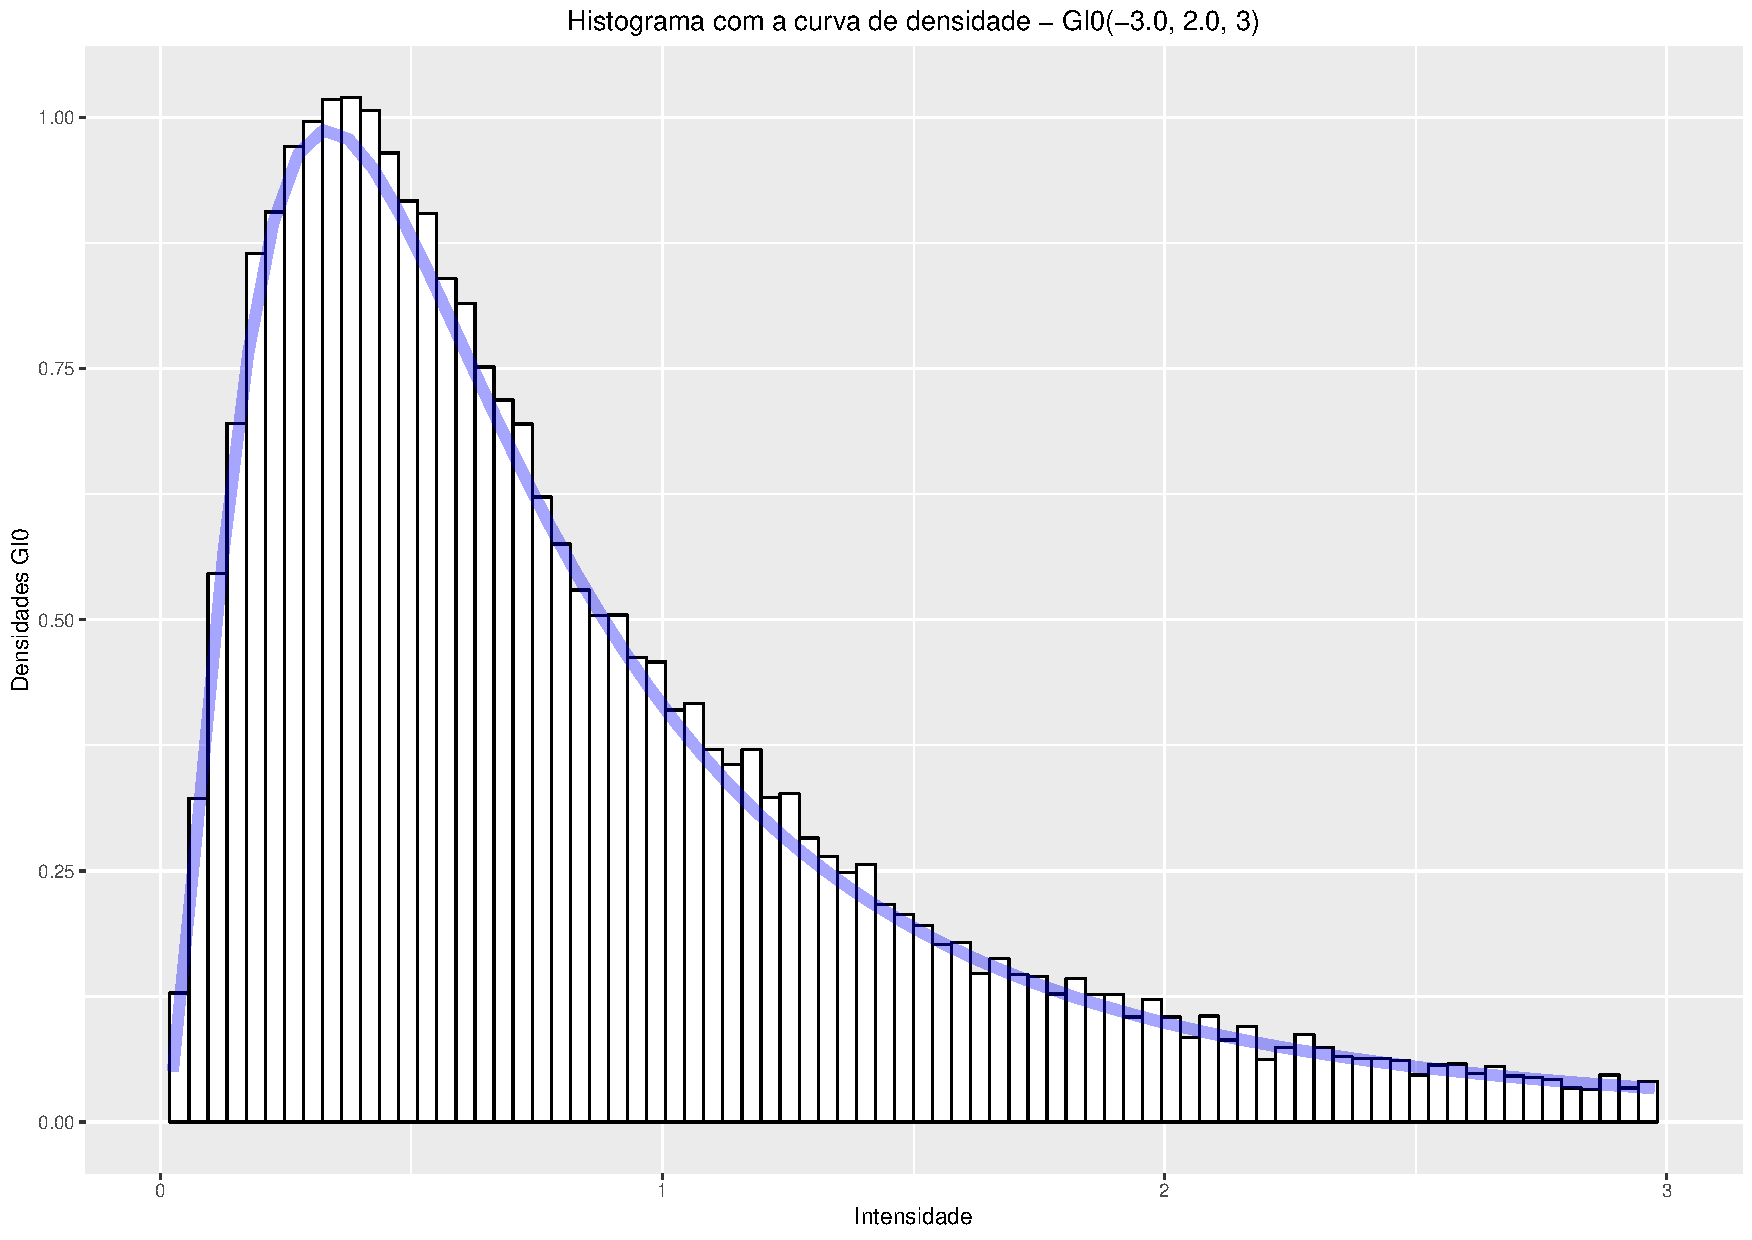
\includegraphics[scale=0.5]{plots/GI0RandVar.pdf}
     \caption{Histograma de variáveis aleatórias $G_I^0(-3.0, 2.0, 3)$ juntamente com sua densidade de probabilidade}
     \label{graf_2}
\end{figure}

Vale reforçar que sistemas que empregam iluminação coerente são usados para explorar regiões inacessíveis e/ou inobserváveis (a superfície de Vênus, o interior do corpo humano, o fundo do mar, áreas sob nebulosidade, etc.). É, portanto, de suma importância poder fazer inferências confiáveis sobre o tipo de alvo em análise, uma vez que informações visuais raramente estão disponíveis.

				
%=========================================================

\section{Introdução à Estatística Inferencial}

Conforme \citet{CasellaBergerStatisticalInference}, uma variável aleatória é caracterizada ou descrita pela sua distribuição de probabilidade. Esta, por sua vez, é descrita pelos seus parâmetros populacionais. Existe um grande interesse em conhecer os parâmetros populacionais da distribuição que se está trabalhando para conhecer como os dados estão se comportando. Como geralmente tais parâmetros não são conhecidos, é preciso desenvolver procedimentos para estimá-los. Desse modo, as estimativas dos parâmetros populacionais são obtidas a partir de variáveis aleatórias de uma amostra representativa da população.
 
As estimativas dos parâmetros populacionais da distribuição são realizadas a partir dos resultados (dados) de uma variável aleatória de uma amostra representativa extraída da população em questão. A esse procedimento damos o nome de estatística inferencial, visto que se está inferindo algo da população a partir de uma amostra populacional.

Existem basicamente duas formas de estimação de parâmetros: por ponto (pontual) ou por intervalo de confiança. De forma breve, a estimativa pontual é um valor obtido a partir dos resultados (dados) de uma variável aleatória de uma amostra representativa da população. Por outro lado, a estimação de parâmetros por intervalo de confiança consiste em gerar um intervalo, centrado na estimativa pontual, no qual se admite que esteja o parâmetro da população.

As técnicas usuais de inferência incluem métodos baseados no princípio de analogia, sendo os estimadores estatísticos de ordem e momento os mais populares desta classe, e no princípio de Máxima Verossimilhança. Entretanto, além dessas técnicas existem os estimadores baseados em Log-Cumulantes ou também chamados de Log-Momentos e os baseados na Teoria da Informação, mais precisamente em Distâncias Estocásticas. Esses dois últimos possuem propriedades bem interessantes e têm sido alvos de pesquisa em diversos trabalhos encontrados na literatura. Neste trabalho, foram estudados e implementados ao todo quatro algoritmos de estimação: Método da Máxima Verossimilhança, Método dos Momentos, Método dos Log-Cumulantes (Log-Momentos) e Método de Distâncias Estocásticas. Nas seções seguintes estão descritas informações a respeito dessas quatro técnicas.

\section{Estimação por Máxima Verossimilhança (MV)}

\subsection{Introdução}

A ideia básica deste método é bem intuitiva. Parece razoável que uma boa estimativa do parâmetro desconhecido \begin{math} \theta \end{math} seria o valor que maximiza a probabilidade de se obter os dados que são observados. É por conta dessa ideia que esse método de estimação é denominado de Máxima Verossimilhança. 
 
Conforme descrito no livro de \citet{CasellaBergerStatisticalInference}, suponha que tenhamos uma amostra aleatória \begin{math} X = (X_{1}, X_{2}, \dots, X_{n}) \end{math} para a qual a função de densidade de probabilidade de cada \begin{math} X_{i} \end{math} é \begin{math} f(x_{i}; \theta)\end{math} 

Então, a função de densidade de probabilidade conjunta da amostra aleatória \begin{math} X \end{math}, denotada por \begin{math} L(\theta) \end{math} é dada por:
\begin{equation}
L(\theta) = P (X_{1} = x_{1} \dots X_{n} = x_{n}) =  f(x_{1}; \theta) \dots f(x_{n}; \theta) =  \prod_{1}^{n} f(x_{i}; \theta)
\end{equation}

A segunda igualdade escrita acima é proveniente do fato de que temos uma amostra aleatória, o que implica, por definição, que cada \begin{math} X_{i} \end{math} seja independente e igualmente distribuída. Agora, à luz da ideia básica da estimação por máxima verossimilhança, uma maneira razoável de proceder é tratar a "função de verossimilhança" dada por \begin{math} L (\theta) \end{math} como uma função de \begin{math} \theta \end{math}, e encontrar o valor do parâmetro que a maximiza.

No contexto das imagens SAR, os estimadores de Máxima Verossimilhança são amplamente utilizados, uma vez que possuem propriedades ótimas bem conhecidas, como consistência, eficiência e normalidade assintótica, entre outras. Por exemplo, esses estimadores foram utilizados para a análise de imagens SAR sob o modelo $K$ no trabalho de \citet{KMaxVer_Joughin}.

\subsection{Estimadores MV para os parâmetros da $G_I^0$}

Então como visto, dado uma amostra $Z = (Z_1, Z_2, \dots, Z_N)$ e assumindo que essas observações são resultados de variáveis aleatórias independentes e identicamente distribuídas que seguem a distribuição $D(\theta)$, com $\theta \in \Theta$, um estimador de Máxima Verossimilhança para $\theta$ é dado por
\begin{equation}
    \widehat{\theta} = \arg\max L(\theta; z) \quad \text{para} \quad \theta \in \Theta, \label{eq:mv}
\end{equation}
em que $L$ é a função de verossimilhança da amostra $Z$ sob o parâmetro $\theta$. Podemos utilizar as propriedades logarítmicas para simplificar os cálculos, aplicando o logaritmo natural, visto que o ponto que produz o máximo da função não varia, independentemente de aplicar ou não o logaritmo. Além disso, sob várias condições é equivalente e muitas vezes mais fácil trabalhar com a função log-verossimilhança reduzida $ \ell (\theta; Z)$, onde todos os termos que não dependem de $\theta$ são ignorados.

Embora a maximização direta de \eqref{eq:mv} seja possível (seja analiticamente ou usando ferramentas numéricas) e desejável, muitas vezes encontramos estimadores de MV resolvendo o sistema de equações (geralmente não-lineares) dado por
\begin{equation}
    \nabla \ell (\widehat{\theta}) = 0 \label{eq:gradient} 
\end{equation}
onde, neste caso, $\nabla$ denota o gradiente. Segundo \citet{FreryMinute2004}, a escolha entre resolver \eqref{eq:mv} ou \eqref{eq:gradient} depende muito de questões computacionais: disponibilidade de algoritmos confiáveis, esforço computacional necessário para implementar e/ou obter a solução e assim por diante. Essas equações, em geral, não têm solução explícita.

Para a construção dos estimadores de Máxima Verossimilhança para o modelo $G_I^0$, considere $Z = (Z_1, Z_2, \dots, Z_N)$ uma amostra aleatória de $N$ variáveis, independentes e igualmente distribuídas, que seguem essa distribuição. Os parâmetros $\alpha$ e $\gamma$ são desconhecidos, enquanto que o parâmetro \textit{Looks} (L) é conhecido. Nesse caso, a função de verossimilhança é $L((\alpha, \gamma); Z) = \prod_{i=1}^{N} f_Z(Z_i)$, onde $f_Z$ é a função densidade de probabilidade definida anteriormente em \eqref{eq:fdpGI0}. 

Assim, a função de log-verossimilhança ($\log L$) é escrita como
\begin{equation}
    \log L((\alpha, \gamma); Z) = N\log \frac{L^{L}\Gamma(L-\alpha)}{\gamma^{\alpha}\Gamma(-\alpha)\Gamma(L)} +  (L-1)\sum_{i=1}^{N}\log Z_i - (L-\alpha)\sum_{i=1}^{N}\log (\gamma + Z_iL) \label{eq:logVer}
\end{equation}

A partir da função acima, podemos escrever a função de log-verossimilhança reduzida, excluindo os termos que não dependem de $\alpha$ e $\gamma$
\begin{equation}
    \ell ((\alpha, \gamma); Z) = N\log\Gamma(L-\alpha) - N\alpha \log\gamma - N\log\Gamma(-\alpha) - (L-\alpha)\sum_{i=1}^{N}\log(\gamma +Z_iL) \label{eq:logVerRed}
\end{equation}

O sistema de equações representado em \eqref{eq:gradient} é, em nosso caso, dado por
\begin{equation}
  \frac{\partial l}{\partial \widehat{\alpha}} = N[\Psi(-\widehat{\alpha}) - \Psi(L-\widehat{\alpha})] + \sum_{i=1}^{N}\log\frac{\widehat{\gamma} + Z_iL}{\widehat{\gamma}} = 0
\end{equation}
\begin{equation}
   \frac{\partial l}{\partial \widehat{\gamma}} = -N\frac{\widehat{\alpha}}{\widehat{\gamma}} - (L - \widehat{\alpha})\sum_{i=1}^{N}(\widehat{\gamma} + Z_iL)^{-1} = 0
\end{equation}
em que $\Psi(\tau) = \frac{\textit{d}log\Gamma(\tau)}{\textit{d}\tau}$ é a função \textit{Digama}. Resolvendo esse sistema de equações obtemos os estimadores para os parâmetros $\alpha$ e $\gamma$ da distribuição $G_I^0$, denotados por $\widehat{\alpha}$ e $\widehat{\gamma}$. Em geral, nenhuma solução explícita para este sistema está disponível e, portanto, rotinas numéricas têm que ser usadas.

Assumindo a simplificação feita para o parâmetro de escala ($\gamma^{*} = -\alpha - 1$), temos que o estimador de Máxima Verossimilhança para o parâmetro $\alpha$, denotado por $\widehat{\alpha}$, é dado pela solução da seguinte equação não linear:
\begin{eqnarray}
    \Psi(-\widehat{\alpha}) - \Psi(L-\widehat{\alpha}) - \log(-\widehat{\alpha}-1) - \frac{\widehat{\alpha}}{\widehat{\alpha}+1} + \nonumber \\ \frac{1}{N}\sum_{i=1}^{N}\log(-\widehat{\alpha} - 1 + LZ_i) - \left ( \frac{\widehat{\alpha}-L}{N} \right )\sum_{i=1}^{N}(-\widehat{\alpha} - 1 + LZ_i)^{-1} & = & 0
\end{eqnarray}

% MOMENTOS 
\section{Estimação pelo Método dos Momentos (MM)}

\subsection{Introdução}

Uma outra forma de encontrar estimadores de parâmetros populacionais, como a média e a variância por exemplo, é através do método dos momentos. Este método é baseado na comparação dos momentos teóricos com os momentos amostrais das variáveis aleatórias envolvidas, a partir de uma amostra de $N$ observações. 

Em suma, o método dos momentos envolve equacionar momentos da amostra com momentos teóricos. Então, vamos começar lembrando as definições dos momentos teóricos, bem como aprender as definições dos momentos das amostras.

A seguir estão algumas definições:

\begin{enumerate}
	\item $E(X^k)$ é o k-ésimo momento teórico da distribuição 
    \item $M_k=\dfrac{1}{N}\sum\limits_{i=1}^N X_i^k$ é o k-ésimo momento amostral 
\end{enumerate}

A ideia por trás desse método é bastante simples. Vejamos os seguintes passos da primeira forma de se calcular os estimadores por este método:
\begin{enumerate}
  \item Equacione o primeiro momento da amostra  $M_1=\dfrac{1}{N}\sum\limits_{i=1}^N X_i=\bar{X}$ ao primeiro momento teórico $E(x)$
  \item Equacione o segundo momento da amostra $M_2=\dfrac{1}{N}\sum\limits_{i=1}^N X_i^2$ ao segundo momento teórico $E(x^2)$
  \item Continuar igualando momentos amostrais, $M_k$, com os correspondentes momentos teóricos  $E(X^k)$, $k = 3, 4, \dots $, até que se tenha tantas equações quanto se tem de parâmetros.
  \item Por fim, basta resolver o sistema e calcular os estimadores para os parâmetros.
\end{enumerate}

Os valores resultantes são chamados de estimadores de método de momentos. Parece razoável que esse método forneça boas estimativas, já que a distribuição empírica converge, em certo sentido, para a distribuição de probabilidade. Portanto, os momentos correspondentes devem ser aproximadamente iguais. Desse modo, estimadores de momentos são favorecidos em aplicações, já que são fáceis de derivar e são, em geral, computacionalmente atraentes. De certo modo, são mais simples de calcular em relação ao método de Máxima Verossimilhança, entretanto podem gerar, com mais frequência, estimadores menos precisos. 

Então, de modo resumido, seja $Z$ uma variável aleatória contínua com função densidade de probabilidade $f_Z(z)$, os momentos teóricos são dados por $m_j = \int x^jf_Z(z)dz$. Os momentos amostrais, por sua vez, são definidos como $\widehat{m_j} = N^{-1}\sum_{i=1}^{N}z_i^j$. Após calcular os momentos teóricos e amostrais, o processo de inferência é simples e consiste em comparar os momentos amostrais, $\widehat{m_j}$, com os correspondentes momentos teóricos, $m_j$, até se ter tantas equações quantos forem os parâmetros a serem estimados. De posse do sistema de equações, basta resolver e calcular os estimadores para os parâmetros. Essa é a ideia geral de funcionamento do Método dos Momentos implementado neste trabalho.

\subsection{Estimadores de Momentos para os parâmetros da $G_I^0$}

Para estimar os parâmetros $\alpha$ e $\gamma$ da distribuição $G_I^0(\alpha, \gamma, L)$, é necessário estimar dois momentos. Neste relatório, serão utilizados momentos de ordem $\frac{1}{2}$ e $1$, ou seja, $m_{1/2}$ e $m_1$ respectivamente. Esses momentos, de acordo com a equação \eqref{eq:moments}, são dados por
\begin{equation}
    m_{1/2} = \left ( \frac{\gamma}{L}\right )^{1/2} \frac{\Gamma(-\alpha-1/2)\Gamma(L+1/2)}{\Gamma(-\alpha)\Gamma(L)} \quad \text{para} \quad \alpha \quad \text{<} \quad -1/2 \label{eq:m12}
\end{equation}
\begin{equation}
    m_{1} = \left ( \frac{\gamma}{L}\right ) \frac{\Gamma(-\alpha-1)\Gamma(L+1)}{\Gamma(-\alpha)\Gamma(L)} \quad \text{para} \quad \alpha \quad \text{<} \quad -1 \label{eq:m1}
\end{equation}

Podemos utilizar o momento $\widehat{m}_{1/2}^2$ para auxiliar nos cálculos e utilizar as equações acima \eqref{eq:m12} e \eqref{eq:m1} para determinar o estimador $\widehat{\alpha}$ que pode ser dado como solução da seguinte equação
\begin{equation}
    g(\widehat{\alpha}) - \zeta = 0
\end{equation}
onde 
\begin{equation}
    g(\widehat{\alpha}) = \frac{\Gamma^2(-\widehat{\alpha} - 1/2)}{\Gamma(-\widehat{\alpha})\Gamma(-\widehat{\alpha} - 1)}
\end{equation}
e
\begin{equation}
    \zeta = \frac{\widehat{m}_{1/2}^2\Gamma(L)\Gamma(L+1)}{\widehat{m}_{1}\Gamma^2(L+1/2)}
\end{equation}
Dessa forma, encontrando o valor de $\widehat{\alpha}$ e o substituindo na equação \eqref{eq:m12} ou na equação \eqref{eq:m1}, obtemos o estimador $\widehat{\gamma}$.

Como já mencionado, podemos simplificar o processo de estimação do parâmetro $\gamma$, obtendo-o este de tal forma que o valor esperado $E(Z^r)$ tenha valor unitário e, assim, definimos ele em função do parâmetro $\alpha$. Como já citado antes o valor de $\gamma^{*}$ vale $-\alpha - 1$. Contudo, abaixo está o cálculo a partir de \eqref{eq:moments} que levou a essa conclusão:
\begin{equation}
    E(Z^r) = 1 \Rightarrow \left (\frac{\gamma*}{L}\right ) \frac{\Gamma(-\alpha-1)\Gamma(L+1)}{\Gamma(-\alpha)\Gamma(L)} = 1 \Rightarrow \gamma* = L\left ( \frac{\Gamma(-\alpha)\Gamma(L)}{\Gamma(-\alpha-1)\Gamma(L+1)} \right ) 
\end{equation}
onde, sabendo que $\Gamma(n) = (n-1)!$, temos
\begin{equation}
    \gamma^{*} = -\alpha - 1
\end{equation}

Estimadores de momentos fracionários foram utilizadas amplamente em \citet{Clutter1997}. Dessa forma, assumindo a simplificação acima e utilizando $r=\frac{1}{2}$ na equação do $r$-ésimo momento da $G_I^0$ dada em \eqref{eq:moments} é preciso resolver a equação a seguir para se obter o estimador de momentos denotado por $\widehat{\alpha}$.
\begin{equation}
    \frac{1}{N}\sum_{i=1}^{N}\sqrt{z_i}-\sqrt{\frac{-\widehat{\alpha} - 1}{L}}\frac{\Gamma(-\widehat{\alpha} - \frac{1}{2})}{\Gamma(-\widehat{\alpha})}\frac{\Gamma(L+\frac{1}{2})}{\Gamma(L)} = 0 \label{fractional_moments}
\end{equation} 

% LOG-CUMULANTES
\section{Estimação pelo Método dos Log-Cumulantes (MLC)}

\subsection{Introdução}

Sabe-se que a estimação de parâmetros de funções de densidade de probabilidade é um dos principais passos na área de processamento de imagens e sinais estatísticos. Nesse contexto, o método de log-cumulantes (MLC) consiste em um método de estimação de parâmetros proposto por \citet{nicolas2002} e tem sido utilizado com resultados satisfatórios em processamentos de imagens SAR.

O Método de Log-cumulantes pode ser visto como uma alternativa às abordagens clássicas de máxima verossimilhança (MV) e método dos momentos (MM). Estudos feitos no trabalho de \citet{krylov2013} derivaram uma condição geral suficiente para uma consistência forte das estimativas de MLC, que representa uma importante propriedade assintótica de qualquer estimador estatístico. Este resultado permite a demonstração da forte consistência das estimativas de MLC para uma seleção de famílias de distribuição amplamente utilizadas originárias de processamento de imagem de radar de abertura sintética, contudo não é restrito somente a esse campo. 

Nesse sentido, estimadores baseados em log-cumulantes têm ganhado espaço na literatura devido às suas boas propriedades e bom desempenho. No contexto de processamento de imagens SAR, este método é especialmente utilizado quando se tem pequenas amostras que se trata de um problema crítico em várias aplicações. Ainda no trabalho de \citet{krylov2013}, foram destacados que os resultados obtidos sugerem que o MLC é uma alternativa viável e computacionalmente rápida que é especialmente útil quando a abordagem direta do estimador de Máxima Verossimilhança se mostra inviável. 

Pesquisadores têm utilizado os parâmetros estimados pelo método de log-cumulantes como entradas, por exemplo, para métodos de classificação de imagens SAR e detecção de mudanças em imagens SAR multitemporais. A seguir é apresentado o MLC conforme proposto e analisado no trabalho de \citet{nicolas2002}.

\subsection{Definição}

Seja $Z$ uma variável aleatória contínua com função densidade de probabilidade $f_Z(z, \theta)$ definida em $\mathbb{R}^{+}$. O Método de log-cumulantes, baseado na transformada de Mellin de $f_Z(z, \theta)$, é definido como:
\begin{equation}
    \phi_{Z}(s) = \int_{0}^{\infty} u^{s-1} f_{Z}(u, \theta)\mathrm{d}u = E(Z^{s-1}) \label{eq:logcum}
\end{equation}
com $s$ sendo um número complexo com norma unitária \citep{nicolas2002}.

Existem dois conceitos importantes para a construção de estimadores utilizando o método de log-cumulantes que são os log-momentos e log-cumulantes de ordem $v$. É possível obter expressões analíticas para os log-momentos e log-cumulantes de ordem $v$ por simples derivações de $\phi_{Z}(s)$, avaliadas em $s = 1$. O log-momento de ordem $v$ pode ser definido como:
\begin{equation}
    \widetilde{m}_{v} = \frac{\mathrm{d}^{v}\phi_{Z}(s)}{\mathrm{d}s^{v}}\Bigr|_{\substack{s=1}} \quad , \quad  v \in \mathbb{N}
    \label{eq:logmomV}
\end{equation}

Tomando como base o logaritmo natural($ln$) de $\phi_{Z}(s)$, pode-se obter o log-cumulante de ordem $v$ de forma bem similar e análoga à equação anterior. Temos que:
\begin{equation}
    \widetilde{k}_{v} = \frac{\mathrm{d}^{v}\psi_Z(s)}{\mathrm{d}s^{v}}\Bigr|_{\substack{s=1}} \quad , \quad  v \in \mathbb{N}
    \label{eq:logcumV}
\end{equation}
com $\psi_Z(s) = \log(\phi_{Z}(s))$.

O funcionamento e estratégia do método de log-cumulantes para estimar o vetor de parâmetros desejado $\theta$ se baseia na relação entre os log-momentos e log-cumulantes que é dada pela seguinte equação:
\begin{equation}
    \widetilde{k}_{v} = \widetilde{m}_{v} - \sum_{i=1}^{v-1}\binom{v-1}{i-1}\widetilde{k}_{i}\widetilde{m}_{v-i}
\end{equation}

Desta equação acima, pode-se destacar como exemplo os log-momentos e log-cumulantes de ordem $1$, $2$ e $3$ que, por sua vez, obedecem a seguinte relação:
\begin{equation}
    \begin{matrix}
        \widetilde{k}_{1} = \widetilde{m}_{1} \\ 
        \widetilde{k}_{2} = \widetilde{m}_{2} - \widetilde{m}_{1}^{2} \\
        \widetilde{k}_{3} = \widetilde{m}_{3} - 3\widetilde{m}_{1}\widetilde{m}_{2} + 2\widetilde{m}_{1}^{3} 
    \end{matrix}  
    \label{eq:logcum123}
\end{equation}

Na maioria das vezes, $\widetilde{k}_{v}$ é calculado como função do vetor de parâmetros $\theta$ e o processo de estimação de $\theta$ é feito substituindo $\widetilde{m}_{v}$ pelo correspondente log-momento amostral, que é dado por:
\begin{equation}
    \widehat{\widetilde{m}}_{v} = \frac{1}{n}\sum_{i=1}^{n}\log z_{i}^{v}
    \label{eq:log_momAmostrais}
\end{equation}
em que $z_i$, $i \in \{1, 2, \dots, n\}$, é uma amostra da variável aleatória $Z$ que segue uma determinada distribuição de probabilidade. A seguir serão mostradas as etapas de construção dos estimadores dos parâmetros da $G_I^0$ mediante utilização do método de log-cumulantes (MLC). 

\subsection{Estimadores MLC para os parâmetros da $G_I^0$}

Para a distribuição $G_I^0$, a função $\phi_{Z}(s)$ é obtida por meio da equação dada anteriormente em \eqref{eq:logcum}, isto é, precisamos utilizar a equação do $r$-ésimo momento da $G_I^0$ dada em \eqref{eq:moments} para obter a expressão para $E(Z^{s-1})$. Portanto, temos:
\begin{equation}
    \phi_{G_I^0}(s) = \left ( \frac{\gamma}{L} \right )^{s-1}\frac{\Gamma(1-s-\alpha)\Gamma(L+s-1)}{\Gamma(-\alpha)\Gamma(L)}  \qquad \alpha \quad \text{<} \quad -s+1
\end{equation}

Utilizando a expressão acima obtida para $\phi_{G_I^0}(s)$ na equação dada em \eqref{eq:logcumV}, obtém-se o seguinte sistema de equações:
\begin{equation}
    \begin{matrix}
        \widetilde{k}_{1} = \log \left ( \frac{\gamma}{L} \right ) + \Psi^{0}(L) - \Psi^{0}(-\alpha)  \\ 
        \widetilde{k}_{2} = \Psi^{1}(L) - \Psi^{1}(-\alpha)
    \end{matrix}
\end{equation}
em que $\Psi^{0}(.)$ e $\Psi^{1}(.)$ correspondem às funções \textit{digama} e \textit{trigama}, respectivamente.

Portanto, para estimar o vetor de parâmetros dado por $\theta = (\alpha, \gamma)^{\top}$ da distribuição $G_I^0$, basta aplicarmos as duas primeiras equações do sistema dado em \eqref{eq:logcum123} que representam os valores de $\widetilde{k}_{1}$ e $\widetilde{k}_{2}$ e as equações encontradas logo acima. Por fim, para estimar os parâmetros, basta substituir os valores de $\widetilde{m}_{1}$ e $\widetilde{m}_{2}$ pelos correspondentes log-momentos amostrais dados pela equação \eqref{eq:log_momAmostrais}. 

Assumindo a simplificação feita de que $\gamma^{*} = -\alpha - 1$, o estimador Log-cumulante do parâmetro $\alpha$ da $G_I^0$ é dado pela solução de $\widehat{\widetilde{k}_{1}} = \log \frac{1-\widehat{\alpha}}{L} + \Psi^{0}(L) - \Psi^{0}(-\alpha)$. Como sabemos que $\widehat{\widetilde{k}}_{1} = \widehat{\widetilde{m}}_{1} = n^{-1}\sum_{i=1}^{n}\log z_i$, então para encontrar o estimador $\widehat{\alpha}$ pelo MLC basta encontrar a solução para:
\begin{equation}
    \frac{1}{n}\sum_{i=1}^{n}\log z_i - \log \left ( \frac{-\widehat{\alpha}-1}{L} \right ) - \Psi^{0}(L) + \Psi^{0}(-\alpha) = 0
    \label{eq:alphaEst_logCum}
\end{equation}

\section{Estimação baseada em Distâncias Estocásticas}

\subsection{Introdução}

Nos últimos anos, houve um crescente interesse em adaptar ferramentas de Teoria da Informação para processamento de imagens. Em particular, o processamento de imagens polarimétricas coerentes também obteve benefícios com esse conceito, uma vez que medidas de divergência podem ser adotadas para fornecer métodos de avaliar algoritmos de segmentação. Ademais, no trabalho de \citet{Goudail:04} a distância de Bhattacharyya foi proposta como um meio de fornecer uma medida de contraste escalar para imagens de SAR polarimétrica e interferométrica.

Nesse contexto, temos que, evidentemente, a teoria da informação tem sido amplamente aplicada à estatística e teoria da probabilidade, obtendo determinado sucesso. \citet{Shannon48} propôs em seu artigo a informação $I(X,Y)$ entre duas variáveis aleatórias $X, Y$ como sendo uma divergência calculada usando as funções de densidade correspondentes $P_{X}, P_{Y}$. Essas divergências foram amplamente estudadas por Kullback e Leibler e Renyi, entre outros autores. Essas divergências têm múltiplas aplicações no processamento de sinal e imagem \citep{Aviyente}, classificação de textura e detecção automática de região em imagens de SAR.

\subsection{Divergências e Distâncias Estocásticas}

Conforme \citet{tese_abraao}, existem diversos parâmetros de separabilidade, que também são comumente chamados de medidas de distância entre distribuições, que possuem o objetivo de determinar se duas distribuições de probabilidade são similares. Nesse contexto, surge o conceito da divergência que se configura justamente como uma medida de distância e cuja definição surgiu com o desenvolvimento da Teoria da Informação. 

De maneira formal, a divergência pode ser definida como uma função não negativa entre duas medidas de probabilidade que obedece as propriedades de definitividade e não negatividade. Se a função também é simétrica, ela é chamada de "distância". Nesse sentido, se a distância também satisfaz a desigualdade triangular, ela é conhecida como "métrica". Por meio do conceito de divergência é que se obtém distâncias entre distribuições de probabilidade. Essas propriedades citadas anteriormente relativa à divergência - definitividade, não negatividade e simetria - são melhor explicadas posteriormente.

Uma imagem pode ser vista como um conjunto de regiões, em que cada uma possui seus pixels descritos por uma variável aleatória que, por sua vez, segue uma determinada distribuição. Assim, \citet{Nascimento2010} propuseram medidas de contraste baseadas em divergências estocásticas para quantificar diferenças entre áreas de imagens SAR. 

Segundo \citet{tese_abraao}, após os primeiros conceitos de divergência, deu-se início ao estudo de classes desta medida. Entre elas pode-se citar a classe de divergências $\phi$ ou família de divergências $\phi$ desenvolvida no trabalho de \citet{Csiszár67}. Esta classe é caracterizada por um procedimento analítico sistematizado e formalizado que permite se obter medidas de divergência a partir da escolha apropriada de uma função convexa $\phi$. Esse estudo foi posteriormente estendido por \citet{salicruetal1993}, no qual foi inserida nesse contexto a função $h$ que permitiu a geração de expressões para uma quantidade maior de divergências conhecidas em relação ao trabalho anterior feito por Csiszár. A nova família de divergências ficou conhecida como família $h - \phi$. 

Sabemos que, por meio de medidas de divergência, é possível se obter expressões para distâncias entre distribuições de probabilidade que, por sua vez, recebem a denominação de distâncias estocásticas ou simplesmente distâncias. De modo geral, uma distância estocástica é uma divergência que além de satisfazer as propriedades de não-negatividade e definitividade, satisfaz a propriedade de simetria. Conforme estudo feito no livro de \citet{StatisticalInferenceBasedonDivergenceMeasures}, a definição formal de distância estocástica será dada a seguir. 
\begin{quote}
    \textbf{Definição de distância estocástica:} Uma distância estocástica definida em um conjunto (domínio) $\nu$ é uma função $ d_\phi^h: \nu \times \nu \rightarrow \mathbb{R} $, onde o contradomínio $\mathbb{R}$ é o conjunto dos números reais, que trata de associar cada par ordenado de elementos $X, Y \in \nu$, que representam variáveis aleatórias, a um número real denotado por $d_\phi^h(X, Y)$. Esta associação é feita de modo que sejam satisfeitas três importantes condições/propriedades para todo e qualquer $X, Y \in \nu$. Tais condições já discutidas anteriormente são descritas a seguir.
    \begin{enumerate}
        \item \textit{Definitividade}: $d_\phi^h(X, Y) = 0 \Leftrightarrow X = Y$;
        \item \textit{Não-Negatividade}: Se $X \neq Y$, então temos $d_\phi^h(X, Y)$ \text{>} $0$;
        \item \textit{Simetria}: $d_\phi^h(X, Y) = d_\phi^h(Y, X)$
    \end{enumerate}
\end{quote}

Um caso particular ocorre quando temos $X$ e $Y$ pertecendo a mesma distribuição de probabilidade, porém com parâmetros diferentes. Nessa situação, é suficiente escrever a notação $d_\phi^h(\theta_1, \theta_2)$. Desse modo, temos que $d_\phi^h(\theta_1, \theta_2) \geq 0$ em que $d_\phi^h(\theta_1, \theta_2) = 0$ se, e somente se $\theta_1 = \theta_2$. Tendo essa igualdade de parâmetros, consequentemente as variáveis $X$ e $Y$ possuem a mesma distribuição e a distância entre elas é nula. Em suma, distâncias estocásticas são utilizadas para comparar e analisar distribuições de probabilidade definidas no mesmo espaço de probabilidades.

\subsection{Introdução à Inferência no contexto da $G_I^0$}

No contexto da estimação de parâmetros, estamos interessados em distâncias entre funções de densidade de probabilidade. Neste trabalho, foi utilizado esse conceito de distância da Teoria da Informação para encontrar o melhor valor para o parâmetro de rugosidade ou textura da distribuição $G_I^0$ - o parâmetro $\alpha$ - de modo que a distribuição empírica de dados seja aproximada pela função de densidade de probabilidade da $G_I^0$. Em outras palavras, a ideia principal consiste de, dada a amostra de dados $z$, calcular $\widehat{\alpha}$, estimador de $\alpha$, como sendo o ponto do espaço paramétrico que minimiza a distância entre a função densidade $f_{G_I^0}$ e uma estimativa da função de densidade subjacente que caracteriza o modelo, isto é, a distribuição empírica dos dados da amostra. O custo computacional de avaliar cada ponto é relativamente pequeno, visto que o histograma está fixado e a densidade não envolve funções especiais. 

Nesse contexto, é possível encontrar o mínimo da distância em função do parâmetro $\alpha$ da $G_I^0$, o qual provê uma forma de estimação do parâmetro. Seja $V$ e $W$ duas variáveis aleatórias definidas sobre o mesmo espaço de probabilidades cujas funções densidade são dadas por $f_V(x; \theta_1)$ e $f_W(x; \theta_2)$. Assim, podemos definir como exemplo as seguintes distâncias estocásticas que são bastante discutidas na literatura:
\begin{enumerate}
    \item \textbf{Distância de Hellinger}: \begin{center} $d_H(V,W) = 1 - \bigint_{-\infty}^{\infty}\sqrt{f_V f_W}$ \end{center}
    \item \textbf{Distância de Bwidehattacharyya}: \begin{center} $d_B(V,W) = -\log\bigint_{-\infty}^{\infty}\sqrt{f_V f_W}$ \end{center}
    \item\textbf{Distância Triangular}: \begin{center} $d_T(V,W) = \bigint_{-\infty}^{\infty}\dfrac{(f_V - f_W)^2}{f_V + f_W}$ \end{center}
    \item \textbf{Distância de Rényi de ordem $\beta$}: \begin{center} $d_R^\beta(V,W) = \dfrac{1}{2(\beta-1)}\log\bigint_{-\infty}^{\infty}(f_V^{\beta}f_W^{1-\beta} + f_V^{1-\beta}f_W^{\beta})$ \end{center}
\end{enumerate}

\citet{Cassetti2013} compararam estimadores baseados nas distâncias acima com o estimador de Máxima Verossimilhança. Os resultados obtidos por esses autores apresentaram evidências de que a Distância Triangular supera as demais e é a melhor escolha para a aplicação testada. \citet{FreryStochasticDistances2015}, por sua vez, focaram seus esforços na estimação de parâmetros para imagens SAR considerando o modelo $G_I^0$ e utilizaram o conceito de Distâncias estocásticas e Kernels Assimétricos para a construção dos estimadores. Se utilizando dos resultados obtidos por \citet{Cassetti2013}, foi implementado um estimador baseado na Distância Triangular. Portanto, neste trabalho, o foco vai ser dado na implementação de um estimador por minimização de distâncias estocásticas utilizando esse tipo de distância.

\subsection{Estimação pela Distância Triangular}

Seja $z = (z_1, z_2, \dots, z_n)$ uma amostra aleatória de $n$ observações independentes distribuídas conforme a distribuição $G_I^0(\alpha_0, \gamma_0^{*}, L_0)$ em que, como já explicado anteriormente, $\gamma_0^{*} = - \alpha_0 - 1$. Uma estimativa para a função de densidade subjacente de $z$ (densidade empírica), denotada por $\widehat{f}$, é utilizada para definir a função objetivo a ser minimizada como uma função do parâmetro $\alpha$. Esta função empírica é calculada a partir do histograma dos dados e utilizando o método de Freedman-Diaconis que pode ser usado para selecionar a largura dos intervalos a serem usados em um histograma. Para um conjunto de medições empíricas amostradas a partir de alguma distribuição de probabilidade, a regra de Freedman-Diaconis \citep{FreedmanDiaconis} é projetada para minimizar a diferença entre a área sob a distribuição de probabilidade empírica e a área sob a distribuição de probabilidade teórica. 

Nesse cenário, o estimador para o parâmetro $\alpha$ baseado na minimização da distância Triangular entre a densidade empírica dos dados $\widehat{f}$ e a densidade do modelo $f_{G_I^0}$, denotado por $\widehat{\alpha}_{T}$, é dado pelo cálculo da seguinte equação:
\begin{equation}
    \widehat{\alpha}_{T} = \arg\min_{-20 \leq \alpha \leq -1} d_T(f_{G_I^0}(\alpha, \gamma_0^{*}, L_0), \widehat{f}(z)) 
    \label{eq: minDT}
\end{equation}
onde $\gamma_0^{*}$ e $L_0$ são previamente conhecidos e $d_T$ é dada pela equação da distância Triangular já descrita anteriormente. Para resolver \eqref{eq: minDT} são requisitadas duas etapas: 1) a integração presente na formula da referida distância utilizando a densidade $G_I^0$ e a densidade estimada $\widehat{f}$ e 2) a otimização com relação ao parâmetro $\alpha$. Vale ressaltar novamente que para solucionar essa equação não há resultados analíticos explícitos, por isso devemos recorrer a procedimentos numéricos. O intervalo de busca é fundamental, sendo estabelecido para evitar instabilidades numéricas nos cálculos realizados.



